\section{Pochodne rożnicowe w przestrzeni}
\begin{frame}{Pochodne rożnicowe w przestrzeni}
	\begin{enumerate}
	\item[(a)] $\frac{d}{dx}$ - informacje o lokalnej zmienności funkcji 
    - sprzęga ze sobą sąsiednie węzły siatki $\newline$
    zamiast $\frac{df}{dx} \Bigm|_j \Rightarrow \textrm{aproksymacja:}$
    \[
    	\Delta x'f_{j}=\frac{f_{j+1}-f_{j-1}}{2\cdot\Delta} \ \
        \textrm{("wycentrowana")}
    \]
    jakość aproksymacji - z porównania:
    $
    \begin{cases}
    	\textrm{- pochodnej zwykłej modu Fouriera} \\
        \textrm{- pochodnej różnicowej modu Fouriera}
    \end{cases}
    \newline
    $
    Mod Fouriera: $u=g_{k}\cdot e^{ikx}$
    \[
    	\frac{du}{dx}=ikg_{k}e^{ikx}=ik\cdot u
    \]
	\end{enumerate}
\end{frame}
%%%%%%%%%%%%%%%%%%%555
\begin{frame}
	\begin{figure}[h]
			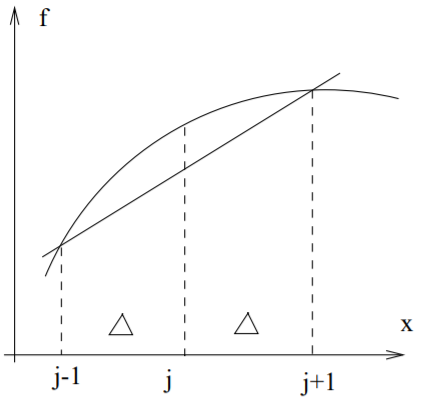
\includegraphics[width=.40\linewidth]{img/20/mrs_img_4}
	\end{figure}
    \[
    	\Delta^{'}_{x}u_{j}=\frac{g_{k}e^{ikx_{j+1}}-
        g_{k}e^{ikx_{j-1}}}{2\cdot\Delta}=\frac{g_{k}e^{ikx_{j}}}
        {2\cdot\Delta}\cdot(e^{ik\Delta}-e^{-ik\Delta})=
    \]
    \[
    	=\frac{i\cdot u}{\Delta}\cdot sin(k\cdot\Delta)=\frac{iu}
        {\Delta}[k\cdot\Delta-\frac{(k\Delta)^{3}}
        {6}+O(k^{5}\Delta^{5})]
    \]
    \[
    	\underbrace{\Delta_{x}'}_{\substack{\textrm{Operator pochodnej} \\ 
        \textrm{różnicowej}}}\ 
        =[1-\frac{(k\Delta)^{2}}{6}+O(k^{4}\Delta^{4})]\ 
        \underbrace{\frac{d}{dx}}_{\textrm{operator pochodnej}}
    \]
\end{frame}
%%%%%%%%%%%%%%%%%%%%%5
\begin{frame}
	Pochodna różnicowa dobrze aproksymuje zwykłą pochodną gdy liczba falowa 
    $k=\frac{2\pi}{L}\cdot l = \frac{2\pi}{\lambda}$ jest mała (dłuższa fala)
    $\newline \newline$
    "wycentrowany" operator $\Delta^{'}_{x}$ - dokładny do wyrazów drugiego 
    rzędu ze względu na $(k \cdot \Delta)^{2}$
\end{frame}
%%%%%%%%%%%%%%%%%%%%%
\begin{frame}
	\begin{enumerate}
    	\item[(b)] $\frac{d^{2}f}{dx^{2}} \rightarrow$ możliwa aproksymacja:
        
	\end{enumerate}
    \begin{figure}[h]
			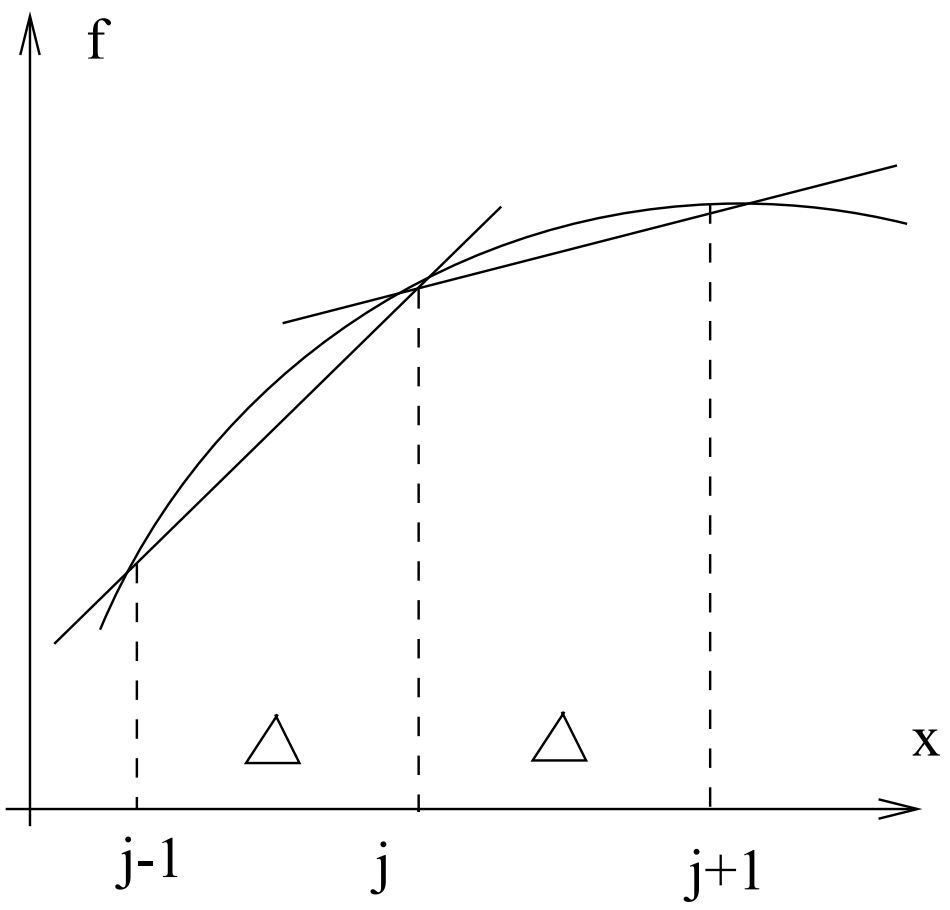
\includegraphics[width=.40\linewidth]{img/20/mrs_img_5}
	\end{figure}
    \[
    	\Delta_{x}''f_{j}=(\frac{f_{j+1}-f_{j}}{\Delta}-\frac{f_{j}-
        f_{j-1}}{\Delta})\cdot\frac{1}
        {\Delta}=\frac{f_{j+1}-2f_{j}+f_{j-1}}{\Delta^{2}}
    \]
    \[
    	\frac{d^{2}u}{dx^{2}}=\frac{d^{2}}{dx^{2}}g_{k}e^{ikx}=-k^{2}\cdot u
    \]
\end{frame}
%%%%%%%%%%%%%%%%%%%%%
\begin{frame}
	\[
    	\Delta{x}''f_{j} = \frac{g_{k}}{\Delta^{2}}
        [e^{ik(x_{j}+\Delta)}-2\cdot e^{ikx_{j}}+e^{ik(x_{j}-
        \Delta)}]=\frac{2u}{\Delta^{2}} [{\it cos} (k\Delta)-1]=
    \]
    \[
    	=\frac{2u}{\Delta^{2}}[1-\frac{k^{2}\Delta^{2}}
        {2}+\frac{k^{4}\Delta^{4}}{24}+O(k^{6}\Delta^{6})-1]=-k^{2}
        u(1-\frac{k^{2}\Delta^{2}}{12}+O(k^{4}\Delta^{4}))
    \]
    \[
    	\underbrace{\Delta_{x}^{''}}_{\substack{\textrm{Operator drugiej} 		\\ 
        \textrm{pochodnej różnicowej}}}\ 
        \ =[1-\frac{k^{2}\Delta^{2}}{12}+O(k^{4}\Delta^{4})]\ 
        \underbrace{\frac{k^{2}}{dx^{2}}}_{\substack{\textrm{Operator 
        drugiej} \\ 
        \textrm{pochodnej}}}
    \]
    $\newline$
    aproksymacja drugiej pochodnej - z dokładnością do wyrazów 2-go rzędu ze
    względu na:
    \[
    	(\frac{2 \pi \cdot \Delta}{\lambda})
    \]
\end{frame}
%%%%%%%%%%%%%%%%%%%%
\begin{frame}{Zastosowanie}
	\begin{block}{}
		Przedstawiona metoda analizy jakości aproksymacji jest przydatna 
        dla:
        \begin{itemize}
        \item pochodnych wyższych rzędow
        \item bardzo złożonych wzorów (operatorów)
        \end{itemize}
	\end{block}
\end{frame}















